\documentclass[oneside,final,a4paper]{report}

\usepackage{graphicx}
\usepackage{enumerate}
\usepackage[parfill]{parskip}
\usepackage[section]{placeins}
\usepackage{listings}

\graphicspath{{../report/images/} {../../www/mte481/website/static/} {./images/}}

\lstset{language=C++}

\oddsidemargin 0in
\evensidemargin 0in
\textwidth 6.5in 

\begin{document}

% ================ Front Matter ================
% Suppress page number for title page and letter of submittal
\pagestyle{empty}

% ==== Title Page
\begin{flushright}
 \begin{LARGE}
  \textbf{UNIVERSITY OF WATERLOO}
 \end{LARGE}

 \begin{large}
  Faculaty of Mechatronics Engineering\\[4cm]
 \end{large}

 \begin{LARGE}
  \textbf{An Obstacle Avoidance System for a}\\
  \textbf{Powered Wheelchair}
 \end{LARGE}

 \vfill

  Prepared By: \\[0.2cm]
  Iain Peet - 20252201\\
  Jordan Valentin - 20271260\\
  Rowan Head-Marsden - 20271527\\
  \today
\end{flushright}
\clearpage

% ==== Letter of Transmittal
\today \\[0.5cm]

Faculty of Mechatronics Engineering \\
University of Waterloo \\
Waterloo, Ontario \\

To Whom It May Concern:

Blah, blah, blah.

Sincerely, \\[1cm]

Iain Peet \hspace{2cm} Jordan Valentin \hspace{2cm} Rowan Head-Marsden
\clearpage

% Resume page numbering
\pagestyle{plain}
\setcounter{page}{1}
\pagenumbering{roman}

% ==== Table of Contents
\setcounter{tocdepth}{1}
\tableofcontents

% ==== List of Figures
\listoffigures
\addcontentsline{toc}{chapter}{List of Tables and Figures}

\chapter*{Executive Summary}
\addcontentsline{toc}{chapter}{Summary}

% ====================== Report Body =================================
\clearpage
\setcounter{page}{1}
\pagenumbering{arabic}
\pagestyle{headings}

\chapter{Introduction}
\section{Background}
Powered wheel chairs have obvious benefits for the mobility of the physically disabled. This can add dramatically to the quality of life for a physically disabled person. Operation of any relatively heavy powered vehicle carries certain safety risks and operators must be capable of safe operation. As a result of safety risks, patients in long-term care facilities are routinely denied the use of powered wheel chairs. 

We spoke with a member of the industy in order to discuss the need for collision-avoidance for powered wheel chairs. Irene Ruel, a physiotherapist in the employ of the British Columbia Interior Health Authority who has previously been responsible for powered wheel chair assessments in an extended care facility, was consulted regarding this problem. By her account, the risk that powered wheelchair operators will collide with other patients is a serious concern and frequently results in the denial of requests for powered wheel chairs for patients living in care facilities. This encouraged our team to develop a wheel chair that helps improve this situation

\section{Need Statement}
Access to powered wheelchairs may be restricted due to concerns regarding a patient's capability for safe operation. A design is needed to assist users in avoiding collisions in order to allow access to powered wheelchairs to a greater number of people.

\section{Objectives and Constraints}
The objectives of this design problem are as follows:

\begin{itemize}
 \item \emph{Improve safety}.  Realistic operating environments will vary greatly in terms of lighting and types of obstacles encoutered, whether static obstacles or moving people/pets. The usefulness of a safety system will be severely degraded if it depends on a specific, controlled environment to be able to operate.
 \item \emph{Improve accessibility}.  For those who would be denied access to a powered wheelchair, a safety system which permits access will have significant quality-of-life benefits.
 \item \emph{Assist with difficult tasks}. Some tasks, such as precise positioning and movement in constrained spaces, are difficult even for unimpaired operators.   A system which can assist with such tasks would be helpful.
\end{itemize}

The constraints of this design are as follows:

\begin{itemize}
 \item \emph{Insensitive to operating environment}.  Realistic operating environments will vary greatly in terms of lighting and types of obstacles encoutered, whether static obstacles or moving people/pets. The usefulness of a safety system will be severely degraded if it depends on a specific, controlled environment to be able to operate.
 \item \emph{Integrates with existsing wheelchairs}.Powered wheelchairs are expensive, but many are already in existence and have been cost-reduced through mass production. Rather than re-inventing the wheel (or wheel-chair in this case) it makes sense to build on existing products by making this an "add-on" feature to an existing chair.

 \item \emph{Cost kept to a minimum}.The system will be paid for by individuals, who will be sensitive to cost. It will be difficult to market a system which is very expensive relative to the cost of a basic powered wheelchair. Initial talks with one pysiotherapist resulted in a suggested cost of not more than \$500 for a system (on top of the base cost of the wheelchair).
\end{itemize}

\section{Criteria}
\begin{figure}[hbt]
 \centering
 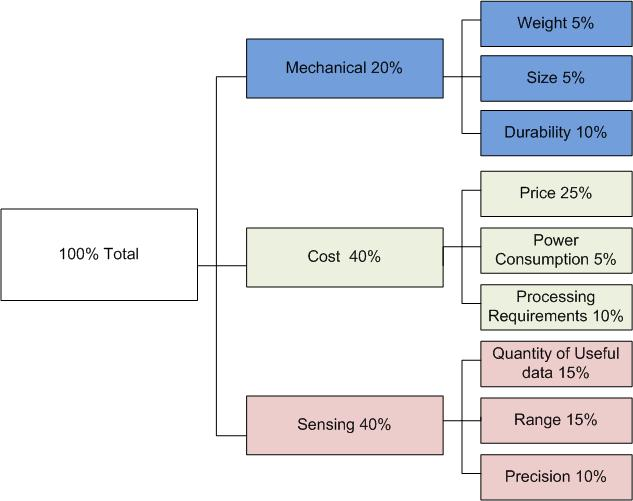
\includegraphics[scale=0.5]{CriteriaWeighting}
 \caption{Criteria Weighting} \label{fig:criteria_weighting}
\end{figure}

\subsection{Weight}
Weight is an important criterion as a number of powered wheel chairs have weight limitations. This should be as small as possible since the weight capacity of a chair like the Invacare Neutron R51LXP is 300 pounds \cite{wheelchair_data}. This means that for any weight we add on to the wheel chair we reduce the potential carrying load of the wheel chair and with it our potential market.

\subsection{Size}
Size is a minor criterion we considered, with an excessively large bulky attachment it would reduce the mobility of the wheel chair and decrease the number of places the wheel chair can travel to. It may also get in the way of the user when operating the wheel chair. This made it important to have some size criteria for measuring the strength of a design.

\subsection{Durability}
While most of the system should not be placed under continuous strain or be at high risk of damage, it is important to consider how durable the design is as there will be wear and tear from use of this system on a wheel chair and damage occurred from movement around the wheel chair.

\subsection{Price}
Price is an important factor for our consideration since we plan to market it to the end users and not to corporations that may have larger budgets. This then made it the most important ranking and with the very large difference in sensor costs it made for a very important factor in determining which route to take.

\subsection{Power Consumption}
Power Consumption measure how much an addition will add to the power consumption of the wheel chair. Many of these chairs are run off of an onboard battery and draining this battery quickly will significantly reduce its usefulness to the users. 

\subsection{Processing Requirements}
The amount of computational intelligence required to handle the data that is coming in from the sensor. This is to make distinction between sensors similar to a Kinect which uses USB and would be plugged into a lab top that will be needed to interpret the data versus something like a sonar sensor that could be tuned and used on FPGA. This will run opposite the Quantity of Useful Data.

\subsection{Quantity of useful Data}
This was selected to distinguish things like sonar which provide simply a distance mapping for a cone versus something like LIDAR, which provides a high-resolution, narrow-beam distance scan. The more data we get from a sensor the more we can make use of it to recognize and avoid obstacles. This runs as the opposite of processing requirements, since more data requires more processing power to interpret the data.

\subsection{Range}
The range for the detection of objects is fairly important to us. While range beyond 7-8 meters is not particularly useful, we want range from about 0 to 8 meters optimally. For this we assume they are working in optimal conditions which we said to be indoors and with normal lighting. Certain sensors we consider have significantly reduced range in other conditions.

\subsection{Precision}
Precision is fairly important since we are detecting obstacles and we would like to know how far away they are, noise and disturbances are acceptable to a small degree so long as we can identify them as noise and not a fast moving obstacle. In addition to this it is important that some sensors have decreased precision at increased range. This is noted as a small reduction in their score.

\section{Design Review}
Design review was achieved internally through group meetings, collaboration, and testing prior to implementing a final section of the project.


\chapter{Electronics and Firmware}

\section{Initial Design}

\section{Final Design}


\chapter{Control Software}

\section{Initial Design}
\begin{figure}[hbt]
 \centering
 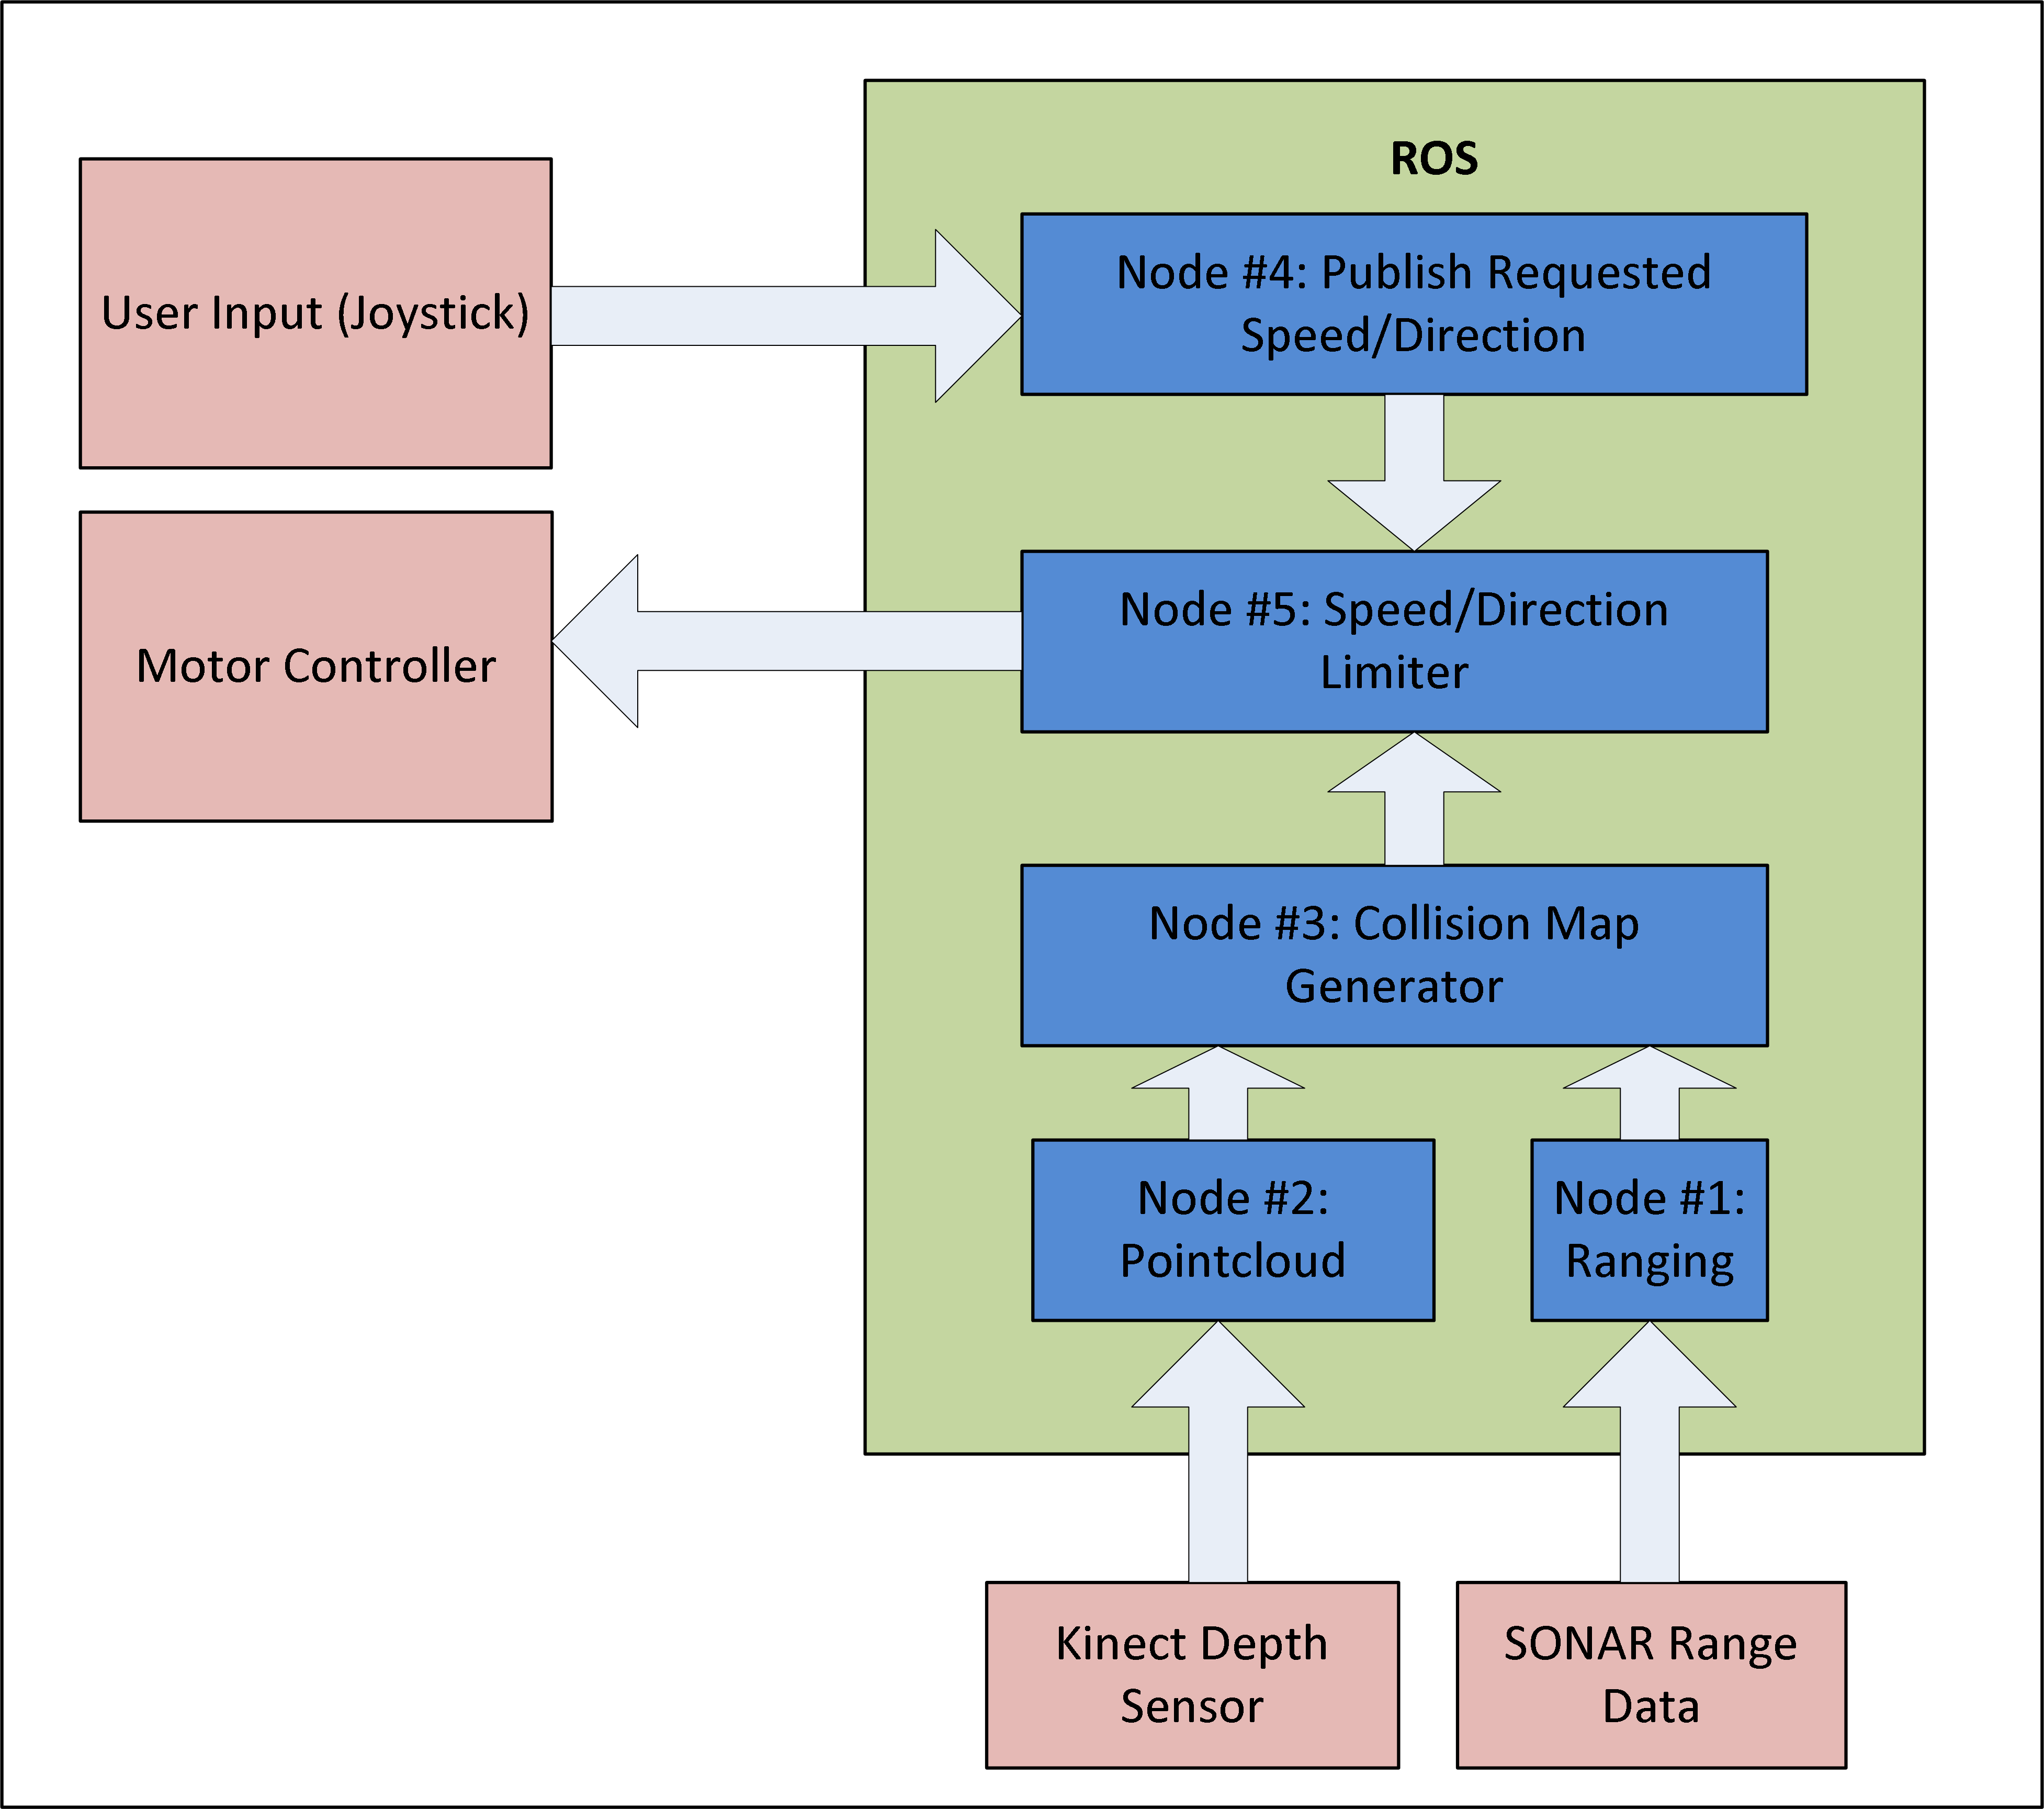
\includegraphics[scale=0.9]{Software_Diagram}
 \caption{Software Design}\label{fig:software}
\end{figure}

Figure \ref{fig:software} shows an overview of the intended software architecture.  Software was intended to be built on the Robot Operating System (ROS) \cite{ROS}, which is a distributed message passing system capable of running on Linux systems.  ROS systems are organized into a network of simple nodes, which co-operate to produce complex aggregate behaviour. 

The following nodes were expected to be required, with the following roles and capabilities:

\subsubsection{Node 1: Ranging}
The ranging node is responsible with communicating with the micro-controller in order to obtain range data from the ultrasonic rangefinders.  It publishes parsed range data.

\subsubsection{Node 2: Point Cloud}
The point cloud node communicates with the Kinect, in order to obtain depth map data.  It publishes point cloud data.

\subsubsection{Node 3: Collision Map Generator}
The collision map generator node is responsible for interpreting poinrt cloud and rangefinder data.  These data are projected into a 2-D occupancy grid in the vehicle frame.  In the simplest case, collision map generation is stateless, and ignores previous data in the interpretation of new sensor data.  If this does not provide sufficient accuracy, the collision map generator might also use state estimates to project old information forward, improving estimates.  

This node subscribes to point cloud and rangefinder data, and publishes collision maps.

\subsubsection{Node 4: Joystick}
The joystick node is responsible for communicating with the joystick, in order to obtain speed and direction commands from the user.  It publishes joystick state.

\subsubsection{Node 5: Speed / Direction Limiter}
The speed / direction limiter node is responsible for communicating with the motor controller in order to set wheel velocities.  It uses a collision map and a wheelchair motion model to assess whether a particular command is likely to lead to a collision.  If necessary, it adjusts user commands in order to avert collisions.

This node subscribes to collision map and joystick command data.  It does not publish anything.

\section{Final Design}
The high-level software architecture has changed substantially since the initial design. Figure \ref{final_arch} shows the block diagram for the implemented system.

\begin{figure}[hbt]
 \centering
 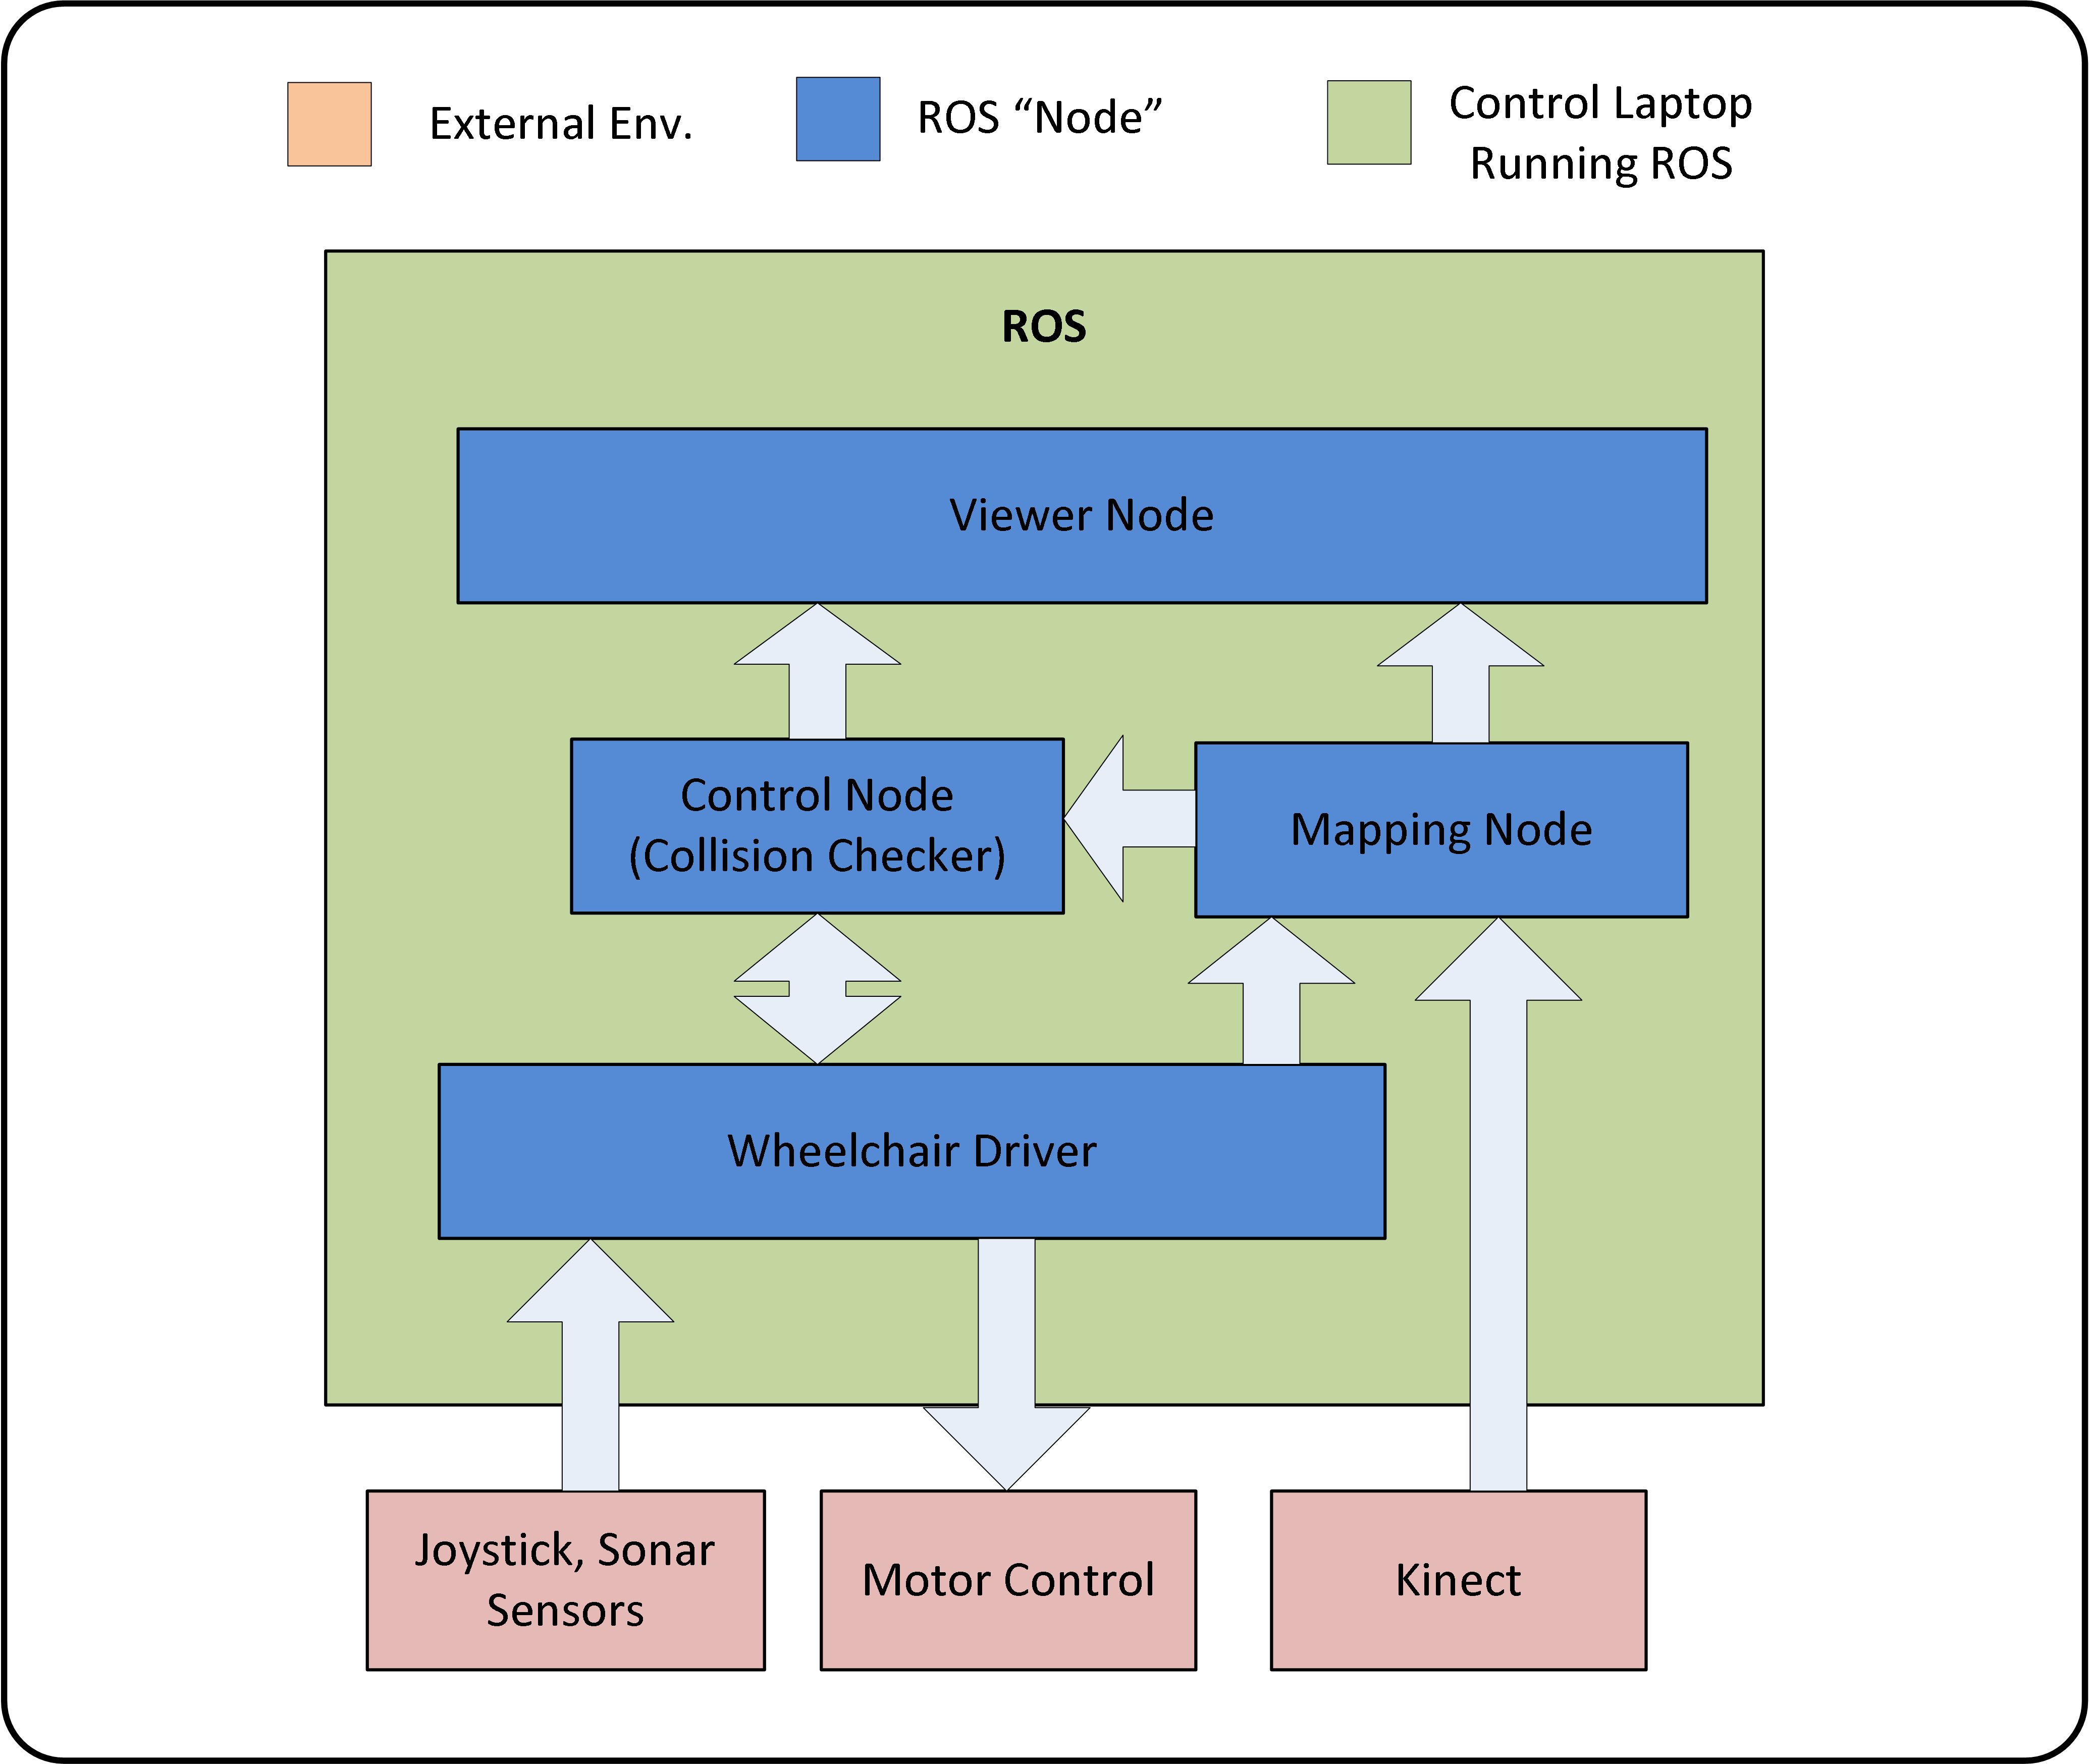
\includegraphics[scale=0.8]{FYDP_Software_Diagram}
 \caption{Final control software architecture}
 \label{final_arch}
\end{figure}


\subsection{ROS Nodes}
The following ROS nodes were included in the final system:

\subsubsection{Wheelchair Driver} 
This node acts as a simple interface between the microcontroller and other ROS nodes.  It has exclusive access to the serial device file associated with the microcontroller, and implements the serial protocol used to send messages to and receive messages from the device.  This node publishes all ranging and joystick input data received from the microcontroller.  It also subscribes to output command messages, which it passes on to the microcontroller.

\subsubsection{Mapping Node} 
This node is responsible for interpreting sensor input in order to produce an occupancy map for the region around the wheelchair.  It subscribes to the sonar range data published by the wheelchair driver, and the pointcloud data published by the off-the-shelf Kinect nodes.  Whenever it receives new data, it computes and publishes a new occupancy grid.

\subsubsection{Control Node}
This node subscribes to the occupancy maps and input commands.  It publishes output commands and trajectory predictions.  It uses a simple model to predict the motion that will result from the input, and checks this path against the occupancy map to predict how soon a collision will occur, if at all.  If the predicted path is safe, the input will be published unmodified as a output command.  If the predicted path is unsafe, the input will be modified in order to prevent collision before being published.

In addition to its normal operation, the control node monitors a parameter value which specifies whether motion is permitted.  If this parameter specifies that motion should be disabled, then the controller node will always publish a zero output.

\subsubsection{Viewer Node}
This node provides a simple user interface for the sytem.  It subscribes to occupancy maps and trajectory predictions.  It uses OpenGL to draw the occupancy map and predicted trajectory, which provides a simple view into the operation of the system.  The viewer node also provides a mechanism for setting the parameter which enables and disables wheelchair motion.

\subsection{Serial Protocol}
The microcontroller and wheelchair driver communicate using a simple, message-based binary protocol.  On the wire, messages have the following structure:

\begin{figure}[hbt]
 \centering
 \begin{tabular}{|l|c|}
  \hline
   Sync Byte 1 & 0xAA \\ \hline
   Sync Byte 2 & 0x55 \\ \hline
   Checksum & 1 byte \\ \hline
   Message Type & 1 byte \\ \hline
   Message Length & 1 byte \\ \hline
   Payload & 0-255 bytes \\ \hline
 \end{tabular}
\end{figure}

The sync bytes are included at the beginning of every message.  Their purpose is to ensure that the microcontroller and wheelchair driver can synchronize if they begin receiving parway through the message, and recover if they lose synchronization due to lost or corrupted data.  The checksum is simply a cumulative XOR combination of all subsequent bytes in the message.  This provides rudimentary error detection capabilities.  The message type indicates to the receiver how the message should be interpreted.  Finally, the message length encodes the length of the payload, which is used in parsing, and is useful for the support of variable-length message types.

Code used to parse messages of this type is shown in \ref{appendix:serial_parsing}.

\subsection{Occupancy Grid}
Kinect pointcloud data and sonar range data are combined to produce an occupancy grid.  

Computation of the occupancy grid from the point cloud is straightforward.  A particular volume of interest is set, and points outside that volume are ignored.  Points within that volume are projected onto a horizontal plane.  Whichever cell they lie in is set to the `occupied state'.

Code which projects the pointcloud into a 2D plane is shown in \ref{appendix:pointcloud_flatten}

It is also fairly simple to obtain an occupancy grid from rangefinder data.  The rangefinders have a wide field of view, so there is significant ambiguity as to the specific location of the object detected by the rangefinder.  In order to represent this, an arc is drawn in the occupancy map, covering the full field of view of the sensor.

Code which draws rangefinder argcs is shown in \ref{appendix:range_occupancy}.

The occupancy maps computed from pointcloud and rangefinder data are then merged using an elementwise logical OR.

\subsection{Trajectory Prediction}
The trajectory of the wheelchair is predicted using an extremely simple motion model, where the forward velocity and angular velocity are taken to be related to the input command by constant coefficients.  This model is described by the following equations:

\begin{equation}
x_t = x_{t-1} + \Delta T K_f u_f \cos (\theta_{t-1})
\end{equation}
\begin{equation}
y_t = y_{t-1} + \Delta T K_f u_f \sin (\theta_{t-1})
\end{equation}
\begin{equation}
\theta_t = \theta_{t-1} + K_{\theta} u_{\theta}
\end{equation}

The forward and angular velocity constants were tuned until they provided reasonable path predictions.

See \ref{appendix:trajectory_prediction} for path prediction code.

\subsection{Collision Detection}
Collision detection is accomplished by checking whether any occupied occupancy grid cells fall within a bounding polygon.  Each of the discrete pose samples along the projected path is tested for collision in this manner.


\chapter{Mechanical}

\section{Initial Design}

\section{Final Design}


\chapter{Project Results}

\section{Prototype Construction}

\section{Test Results}

\chapter{Schedule and Budgeting}

\section{Original Schedule}

\section{Actual Schedule}

\section{Budget}

\section{Actual Cost}


\chapter{Conclusions and Recommendations}

% Set special section numbering for appendices
\renewcommand{\thesection}{A\thechapter.\arabic{section}}

\chapter*{Appendix A - Selected Control Software Code Listings}
Complete source code can be obtained at http://github.com/ipeet/mte481

\setcounter{chapter}{1}
\addcontentsline{toc}{chapter}{Appendix A - Selected Code Listings}
\section{Serial Protocol Parsing State Machine}
Excerpt from common/serial/protocol.c
\label{appendix:serial_parsing}
\begin{lstlisting}
 // Parse a new byte
enum ParseStatus pr_push(uint8_t byte) {
  if (_state == DONE) {
    // start reading a new message
    pr_init();
  }

  switch (_state) {
    case SYNC_1:
      if (byte == SYNC_BYTE_1) {
        _state = SYNC_2;
        return OK;
      } else {
        return BAD_SYNC;
      }

    case SYNC_2:
      if (byte == SYNC_BYTE_2) {
        _state = CHECKSUM;
        return OK;
      } else {
        pr_init();
        return BAD_SYNC;
      }

    case CHECKSUM:
      _buf.checksum = byte;
      _state = TYPE;
      return OK;

    case TYPE:
      _buf.type = byte;
      _state = LENGTH;
      return OK;

    case LENGTH:
      _buf.length = byte;
      if (byte == 0) {
        _state = DONE;
        break;
      } else {
        _payloadBytes = 0;
        _state = PAYLOAD;
        return OK;
      }

    case PAYLOAD:
      _buf.raw[_payloadBytes] = byte;
      _payloadBytes++;
      if (_payloadBytes < _buf.length) {
        return OK;
      } else {
        _state = DONE;
        break;
      }
    
    default:
      pr_init();
      return INVALID;
  };

  // Should only fall through for checksum on a complete package
  if (_state != DONE) return INVALID;

  /* Validate checksum */
  if (pr_checksum(&_buf) == _buf.checksum) {
    return COMPLETE;
  } else {
    return BAD_CHECKSUM;
  }
}
\end{lstlisting}

\clearpage
\section{Projection of a Pointcloud Into an Occupancy Grid}
Excerpt from wheelchair\_ros/src/occupancy.cpp
\label{appendix:pointcloud_flatten}
\begin{lstlisting}
void Occupancy::handlePointcloud(const PointCloud::ConstPtr &msg) {
  /* Convenience */
  int w = m_width / m_resolution;
  int d = m_depth / m_resolution;
  int h = m_height / m_resolution;

  m_kinect2d.clear();
  m_kinect2d.resize(w*d);

  m_kinect3d.clear();
  m_kinect3d.resize(w*d*h);

  for (unsigned i=0; i < msg->points.size(); ++i) {
    double x = msg->points.at(i).x;
    double y = -msg->points.at(i).y;
    double z = msg->points.at(i).z;

    /* Bounds check the point */
    if (isnan(x) || isnan(y) || isnan(z)) continue;
    int xi = (x - m_orig_x) / m_resolution;
    int yi = (y - m_orig_y) / m_resolution;
    int zi = (z - m_orig_z) / m_resolution;
    if (xi < 0) continue;
    if (xi >= w) continue;
    if (yi < 0) continue;
    if (yi >= h) continue;
    if (zi < 0) continue;
    if (zi >= d) continue;
    m_kinect2d[zi*w + xi] = 100;
    m_kinect3d[yi*d*w + zi*w + xi] = 1;
  }
}
\end{lstlisting}

\clearpage
\section{Computation of an Occupancy Grid from Rangefinder Data}
\label{appendix:range_occupancy}
Excerpt from wheelchair\_ros/src/occupancy.cpp
\begin{lstlisting}
void Occupancy::handleSonar(const Sonar::ConstPtr &msg) {
  /* Convenience */
  int w = m_width / m_resolution;
  int d = m_depth / m_resolution;
  int h = m_height / m_resolution;

  m_sonar2d.clear();
  m_sonar2d.resize(w*d);

  m_sonar3d.clear();
  m_sonar3d.resize(w*d*h);

  for (int i=0; i<4; ++i) {
    for (double j=-0.5*config::SONAR_FOV; j < 0.5*config::SONAR_FOV; j+=0.02) {
      pair<double, double> pos = m_sonars[i].inOccupancy(
          *this, msg->ranges[i], j);
      double x = pos.first;
      double z = pos.second;
      int xi = (x - m_orig_x) / m_resolution + 0.5;
      int zi = (z - m_orig_z) / m_resolution + 0.5;
      if (xi < 0) continue;
      if (xi >= w) continue;
      if (zi < 0) continue;
      if (zi >= d) continue;
      m_sonar2d[zi*w + xi] = 100;
      m_sonar3d[zi*w + xi] = 1;
    }
    m_ranges[i] = msg->ranges[i];
  }
  m_haveSonar = true;
}

pair<double, double> Occupancy::SonarPose::inOccupancy
  (const Occupancy &occ, double rad, double ang) 
{
  if (rad < 3*config::RESOLUTION) {
    rad = 3*config::RESOLUTION;
  }
  double x = m_x + rad * cos(ang + m_dir);
  double y = m_y + rad * sin(ang + m_dir);
  return pair<double, double> (x, y);
}
\end{lstlisting}

\clearpage
\section{Trajectory Prediction}
\label{appendix:trajectory_prediction}
Excerpt from wheelchair\_ros/src/controller.cpp

\begin{lstlisting}
PredictedPath::Ptr Controller::predictPath(const Twist::ConstPtr &input) {
  PoseStamped::Ptr curState (new PoseStamped);
  curState->pose.position.x = 0;
  curState->pose.position.y = 0;
  curState->pose.position.z = 0;
  curState->pose.orientation.x = 0;
  curState->pose.orientation.y = 0;
  curState->pose.orientation.z = 1;
  curState->pose.orientation.w = 0.5*M_PI;

  PredictedPath::Ptr ret (new PredictedPath);
  ret->poses.push_back(*(curState));
  ret->poseCollides.push_back(false);
  ret->timestep = config::TIMESTEP;
  for (double t=0; t <= config::SIM_LENGTH; t += config::TIMESTEP) {
    curState = predict(curState, input, config::TIMESTEP);
    ret->poses.push_back(*curState);
    double curX = curState->pose.position.x;
    double curY = curState->pose.position.y;
    bool col = collides(curX, curY, curState->pose.orientation.w);
    ret->poseCollides.push_back(col);
    if (col) break;
  }
  return ret;
}

PoseStamped::Ptr Controller::predict(
    PoseStamped::Ptr prev, const Twist::ConstPtr &input, double step) 
{
  PoseStamped::Ptr ret (new PoseStamped);

  // Initialize values from motion-in-plane assumption:
  ret->pose.position.z = 0;
  ret->pose.orientation.x = 0;
  ret->pose.orientation.y = 0;
  ret->pose.orientation.z = 1;

  // Compute current velocities:
  double angular = config::K_ROT * (-input->linear.x + config::LAT_OFFSET);
  double forward = config::K_FWD * (input->linear.y - config::FWD_OFFSET); 
  double heading = prev->pose.orientation.w; // convenient

  // Forward difference computation of next state:
  ret->pose.orientation.w = heading + step * angular;
  ret->pose.position.x = 
    prev->pose.position.x + forward*cos(heading);
  ret->pose.position.y =
    prev->pose.position.y + forward*sin(heading);

  return ret;
}
\end{lstlisting}

\begin{thebibliography}{9}
 \addcontentsline{toc}{chapter}{Bibliography}
 \bibitem{patent:computer_controlled}
  L. Fehr, S. Skaar, G. Del Castillo. \\
  \emph{Computer Controlled Power Wheelchair Navigation System.} \\
  U.S. Patent 2008/7383107B2, Jun. 3, 2008.
 \bibitem{patent:power_wheelchair}
  G. Griggs, T. Dutta, G. Fernie. \emph{Powered Wheelchair},\\
  U.S. Patent 2010/0082182A1, Apr. 1, 2010.
 \bibitem{patent:wheelchair_method}
  T. Smithers, U. Urriticoechea, U. Campos. \\
  \emph{Wheelchair and Method for Correcting the Guidance of a Wheelchair.} \\
  U.S. Patent 2011/0130940A1, Jun. 2, 2011.
 \bibitem{NASA}
  NASA. \emph{NASA-STD-3000. Anthropometry and Biomechanics.}\\
  http://msis.jsc.nasa.gov/sections/section03.htm, Jul. 1995.
\bibitem{primesense}
  \emph{Our Full 3D Sensing Solution}, \\
  \mbox{http://www.primesense.com/en/technology/115-the-primesense-3d-sensing-solution} \\
  2011.
 \bibitem{OpenNI}
  http://www.openni.org/
 \bibitem{ROS}
  http://www.ros.org/
 \bibitem{point_clouds}
  http://pointclouds.org/
 \bibitem{wheelchair_data}
  Invacare. \emph{Nutron R51LXP. Invacare Product Catalogue.} \\
  http://www.invacare.ca/cgi-bin/imhqprd/inv\_catalog/prod\_cat\_detail.jsp?s=0\&prodID=R51LXP\\
 Jan. 2011.
\bibitem{kinect_prec}
  L. Yiping. \\
  \emph{openni\_kinect/kinect\_accuracy}, http://www.ros.org/wiki/openni\_kinect/kinect\_accuracy\\
  Jun. 27, 2011.
 \bibitem{lv-ez4}
  MaxBotix Inc, \emph{LV-EZ4 Datasheet},  2011
 \bibitem{lv-ez0}
  MaxBotix Inc, \emph{LV-EZ0 Datasheet},  2011
 \bibitem{kinect_power}
  M. Wise.  \emph{Adding a Kinect to an iRobot Create} \\
  http://www.ros.org/wiki/kinect/Tutorials/Adding\%20a\%20Kinect\%20to\%20an\%20iRobot\%20Create\\
  May 2, 2011.
 \bibitem{MSP430_USB}
  A. Dannenberg. (2006, October). \emph{MSP430 Connectivity Using TUSB3410},\\
  http://www.ti.com/lit/an/slaa276a/slaa276a.pdf
\end{thebibliography}

\end{document}